\documentclass[10pt]{article}
\usepackage[margin=0.60in]{geometry}
\usepackage{booktabs,enumitem,fancyhdr,graphicx,listings,tabularx,titlesec,xcolor}
\usepackage[hidelinks]{hyperref}
\graphicspath{{docs/lessons/assets/}{../assets/}}
\hypersetup{
 pdftitle={ADK Lesson 060: Dual-Display Timing Desk},
 pdfauthor={Kevin Shanahan},
 pdfsubject={Deterministic stopwatch control, coherent dual-display presentation, copied acknowledgements, and disagreement handling},
 pdflang={en-US}}
\pagestyle{fancy}\fancyhf{}
\lhead{\textsc{ADK Lesson 060}}\rhead{Dual-Display Timing Desk}
\cfoot{\thepage}\setlength{\headheight}{14pt}
\setlength{\parindent}{0pt}\setlength{\parskip}{3pt}
\setlist{nosep,leftmargin=1.45em}
\titleformat{\section}{\Large\bfseries}{\thesection}{0.5em}{}
\newcommand{\lessonbox}[1]{\begin{center}\fbox{\parbox{0.92\linewidth}{#1}}\end{center}}
\newcommand{\blankline}{\rule{0.76in}{0.4pt}}
\newcommand{\longblank}{\rule{1.28in}{0.4pt}}
\lstset{
 basicstyle=\ttfamily\footnotesize,
 columns=fullflexible,
 breaklines=true,
 frame=single,
 rulecolor=\color{black},
 showstringspaces=false}

\begin{document}
\small
\begin{center}
 {\Huge\bfseries Dual-Display Timing Desk}\\[3pt]
 {\Large Keep one stopwatch story coherent across two independent presenters}\\[7pt]
 \fbox{\textbf{E0 COPIED POLICY REPLAY --- ZERO DISPLAY HARDWARE}}
\end{center}
\begin{tabularx}{\linewidth}{@{}>{\bfseries}l X >{\bfseries}l X@{}}
Lesson & 060 --- project & Time & 180--240 minutes\\
Prerequisites & Lessons 058--059 & Board & compile-only Mega replay\\
Capacity & one stopwatch and one pending presentation & Observation & named memory result cells\\
\end{tabularx}

\lessonbox{\textbf{Responsibility.}
\texttt{DualDisplayTimingDesk} owns deterministic stopwatch state, copied
control admission, one immutable presentation snapshot, two generation-bound
display intents, self-test progress, and disagreement provenance. It owns no
button, pin, timer, interrupt, bus, display, module, supply, clock, retry loop,
or powered circuit.}

\section{Build one story, not two clocks}
The timing desk presents the same stopwatch snapshot in two different ways.
Four digits show minutes, seconds, and tenths. An eight-by-eight matrix shows a
perimeter dial and a central status glyph. Those outputs are generated
independently, so Lesson 060 must preserve the shared meaning before either
child policy begins its own service sequence.

\begin{center}
% ADK visual: pencil
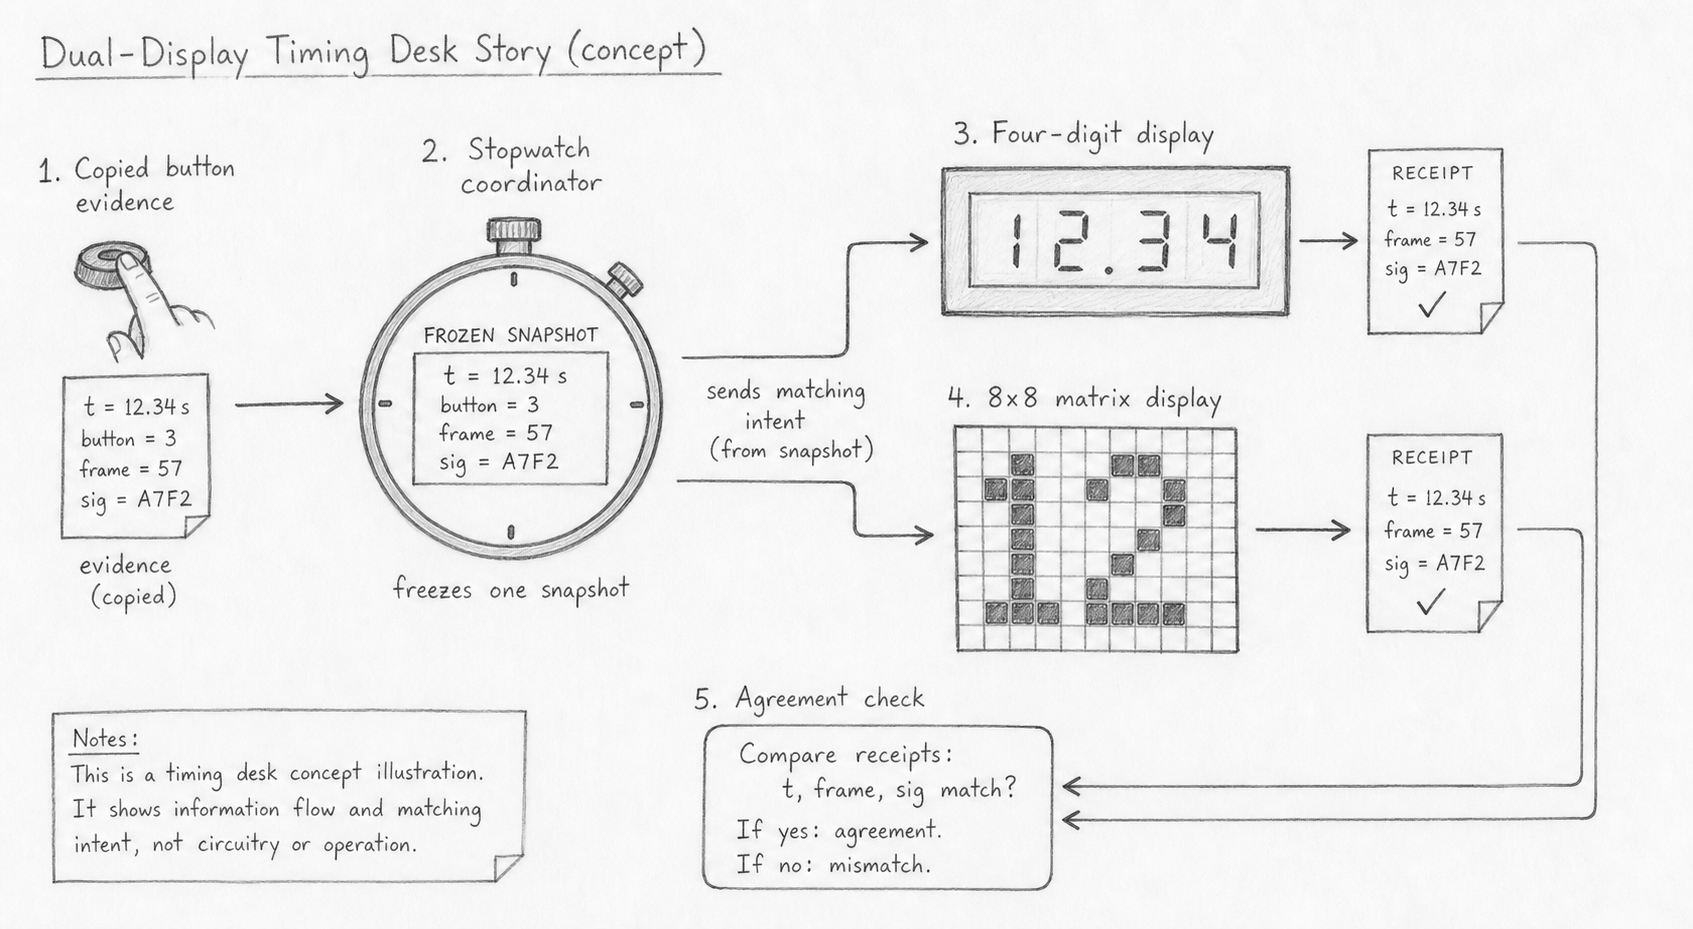
\includegraphics[width=0.95\linewidth,height=2.10in,keepaspectratio]
 {060-one-story-pencil.png}

\small\textit{Alternative text: a pencil-drawn stopwatch snapshot card forks
into a four-digit time card and an eight-by-eight dial card; both cards carry
the same nonzero presentation generation while two independent service paths
continue below.}
\end{center}

Atomic presentation means that both children receive values derived from one
immutable logical snapshot. It does not mean simultaneous photons, a
rollback-capable MAX7219 transport, or proof that either display changed.

\begin{tabularx}{\linewidth}{@{}X X@{}}
\toprule
E0 proves & E0 does not prove\\
\midrule
one copied stopwatch snapshot feeds both intents & both displays changed at the same instant\\
both previews pass before either pure commit & physical writes can roll back\\
accepted logical frame receipts match expected values & LEDs were visible or optically agreed\\
bounded supplied-time behavior & an interrupt or hardware timer met deadlines\\
\bottomrule
\end{tabularx}

\section{Admit copied controls before changing time}
The project consumes copied start/pause, lap, and reset evidence. Each envelope
must carry the expected source identity, configuration revision, sequence,
observation time, and consistent edge and level facts. Structural validation
happens before reset precedence, so a reset bit cannot smuggle malformed
companion evidence into the state machine.

Reset dominates every valid simultaneous control. Without reset, simultaneous
start/pause and lap presses are ambiguous and do not mutate the stopwatch.
Held levels do not repeat; only admitted edges act.

\begin{center}
% ADK visual: pencil
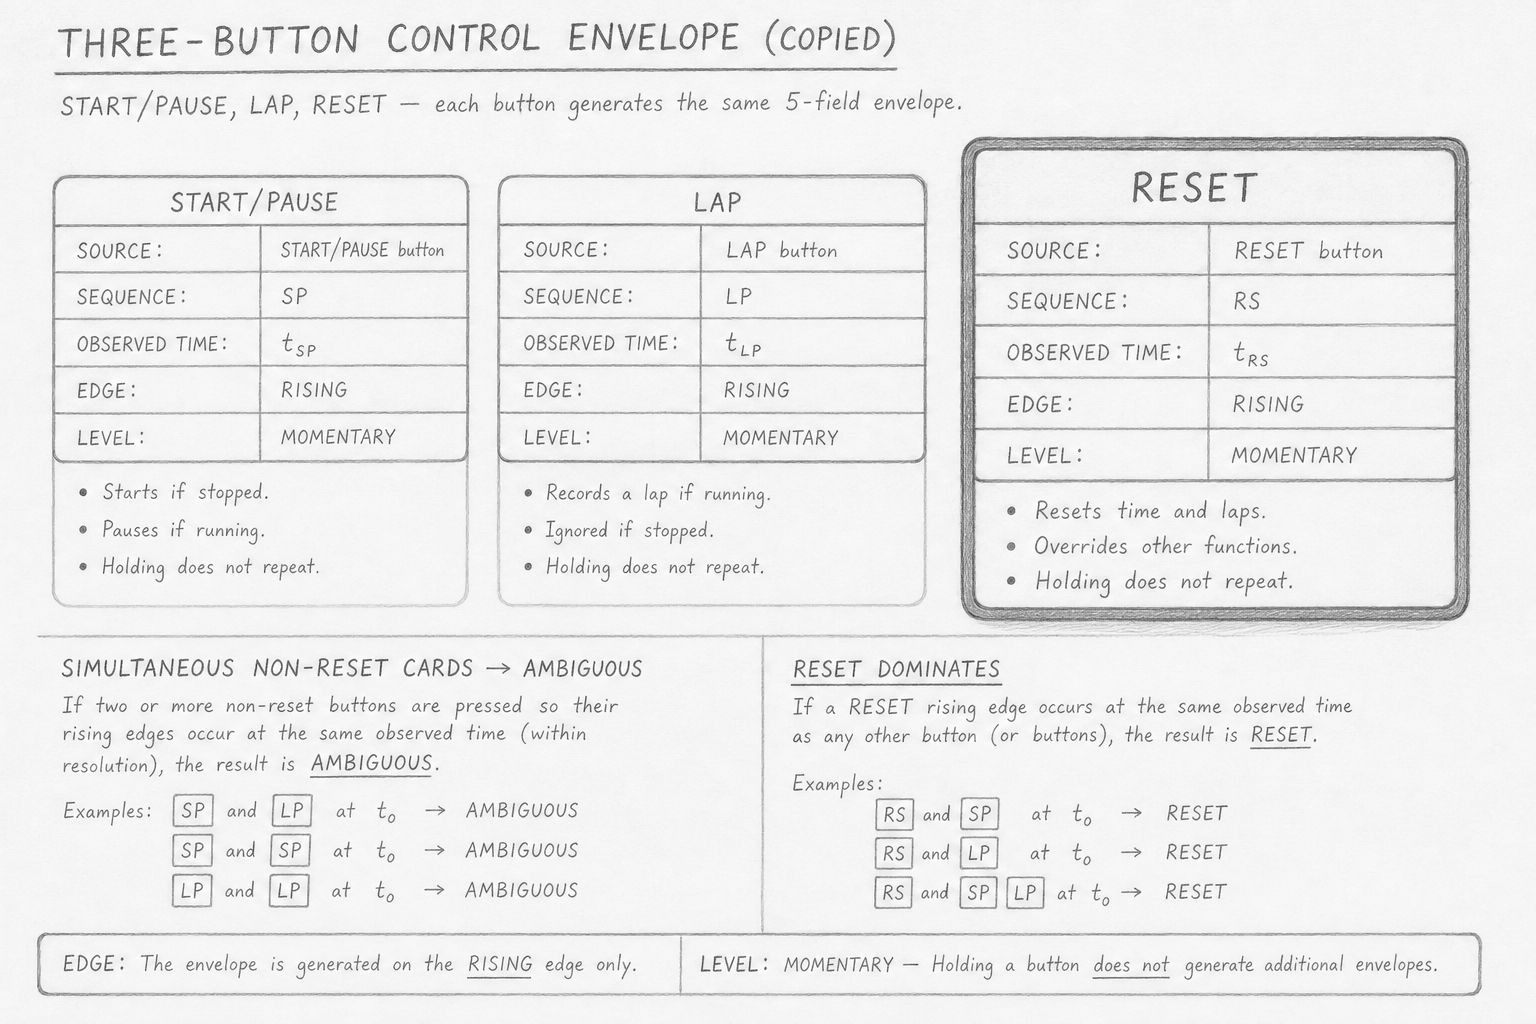
\includegraphics[width=0.94\linewidth,height=1.95in,keepaspectratio]
 {060-control-envelope-pencil.png}

\small\textit{Alternative text: three pencil button cards enter a validation
gate carrying identity, sequence, time, edge, and level fields;
after the gate, reset takes the upper dominant path while a simultaneous
non-reset pair enters an ambiguity box without changing stopwatch state.}
\end{center}

\begin{tabularx}{\linewidth}{@{}l l X@{}}
\toprule
Valid edge set & Result & Reason\\
\midrule
reset plus anything & stopped at canonical zero & reset dominance\\
start/pause only & start, pause, or resume & phase-dependent toggle\\
lap only while running & copy current elapsed for a timed hold & stopwatch continues internally\\
start/pause plus lap & no stopwatch mutation & ambiguous non-reset intent\\
no edge; held level & no repeated action & edges act once\\
\bottomrule
\end{tabularx}

Before replay, predict whether a structurally invalid envelope containing a
reset edge can clear a fault: \longblank. Then explain which validation rule
supports your answer: \longblank.

\section{Derive elapsed time only from supplied time}
The stopwatch phases are stopped-zero, running, paused, and faulted. Running
elapsed time is derived from supplied \texttt{TimePoint} values. Pause
materializes elapsed time; resume continues from that materialized value. Lap
copies the current elapsed value without stopping the internal clock.

Capacity is \(9{:}59.9\). Reaching capacity saturates visibly and stops rather
than wrapping. Backward time and an exact unsigned half-range difference
reject atomically.

\begin{center}
% ADK visual: pencil
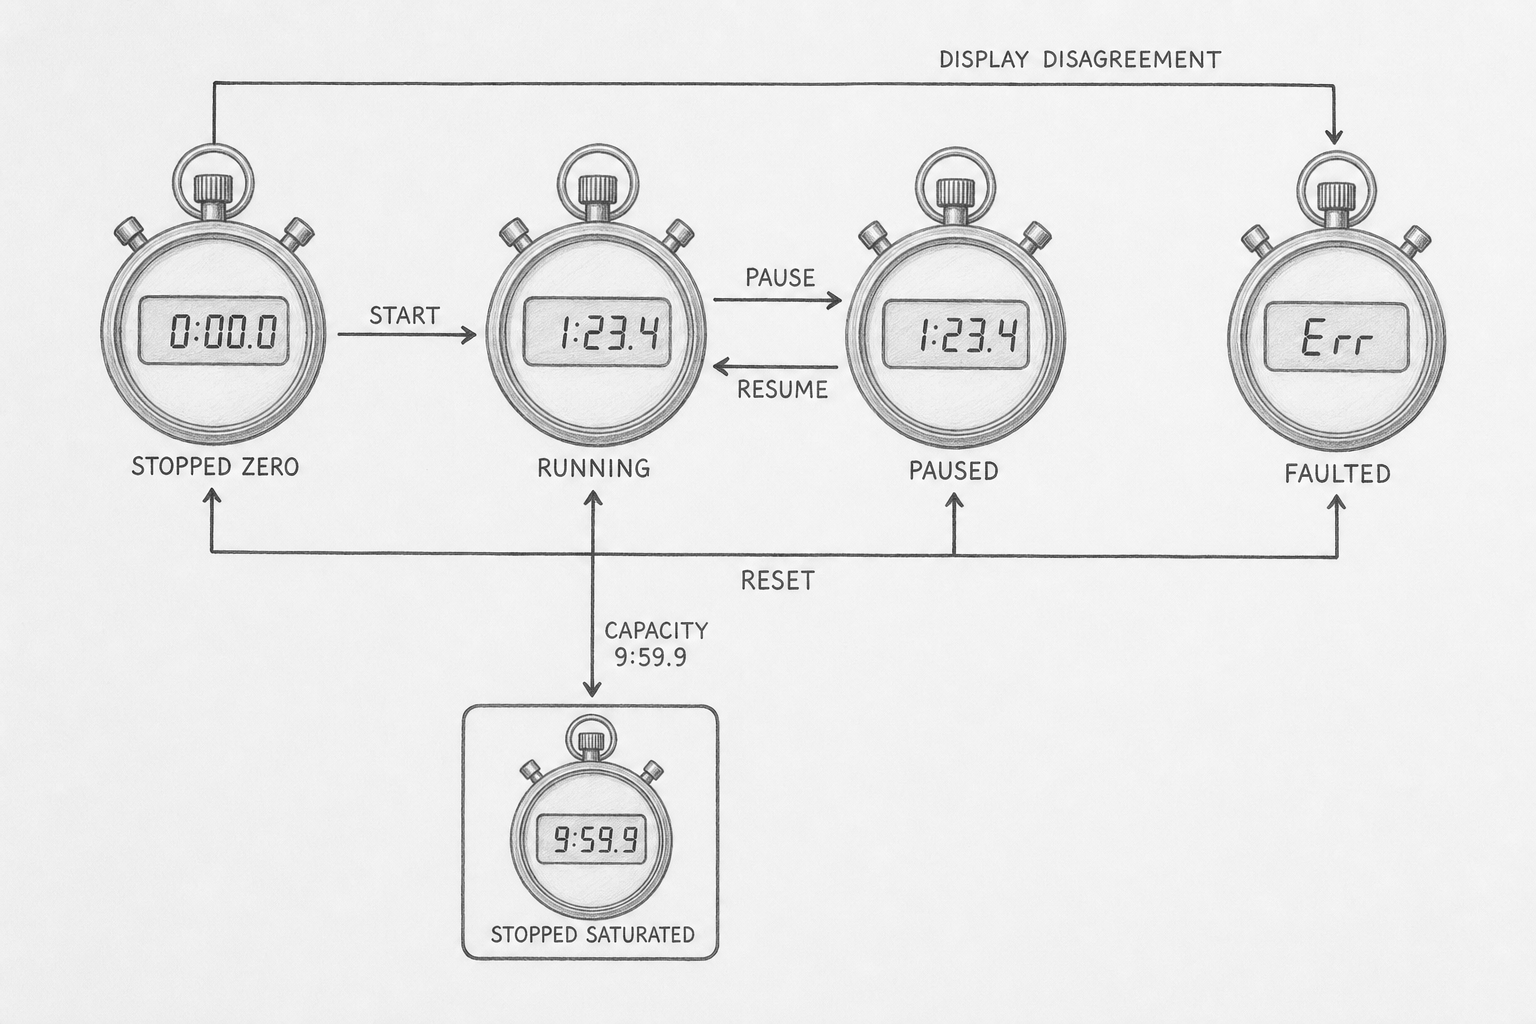
\includegraphics[width=0.96\linewidth,height=1.85in,keepaspectratio]
 {060-stopwatch-states-pencil.png}

\small\textit{Alternative text: a hand-drawn state map connects stopped zero,
running, and paused with start-pause edges; a lap tracing sheet overlays
running without stopping it, reset returns every valid state to zero, and the
capacity boundary leads to a saturated stopped card.}
\end{center}

\begin{tabularx}{\linewidth}{@{}l X X@{}}
\toprule
Boundary & Prediction & Evidence to inspect\\
\midrule
start at zero & running with zero elapsed & phase and anchor time\\
pause at 12,345 ms & paused at copied elapsed & materialized elapsed\\
resume, then lap & running continues behind frozen presentation & current and lap snapshots\\
reach 599,900 ms & show \(9{:}59.9\), then stop & saturation and phase\\
time regression & no accepted state changes & control status and prior snapshot\\
\bottomrule
\end{tabularx}

\section{Map the ordinary digit frame}
Elapsed time renders left to right as minute, seconds tens, seconds units, and
tenths. Decimal mask \texttt{0x0A} lights the separator after the minute and
the separator after the seconds units. Stopped and running show current
elapsed time; paused shows materialized elapsed.

A lap press freezes both presentation frames at the lap snapshot for exactly
2,000 ms while a running stopwatch continues internally. The inclusive
deadline still shows the lap. The next valid tick returns presentation to
current time.

\begin{center}
% ADK visual: pencil
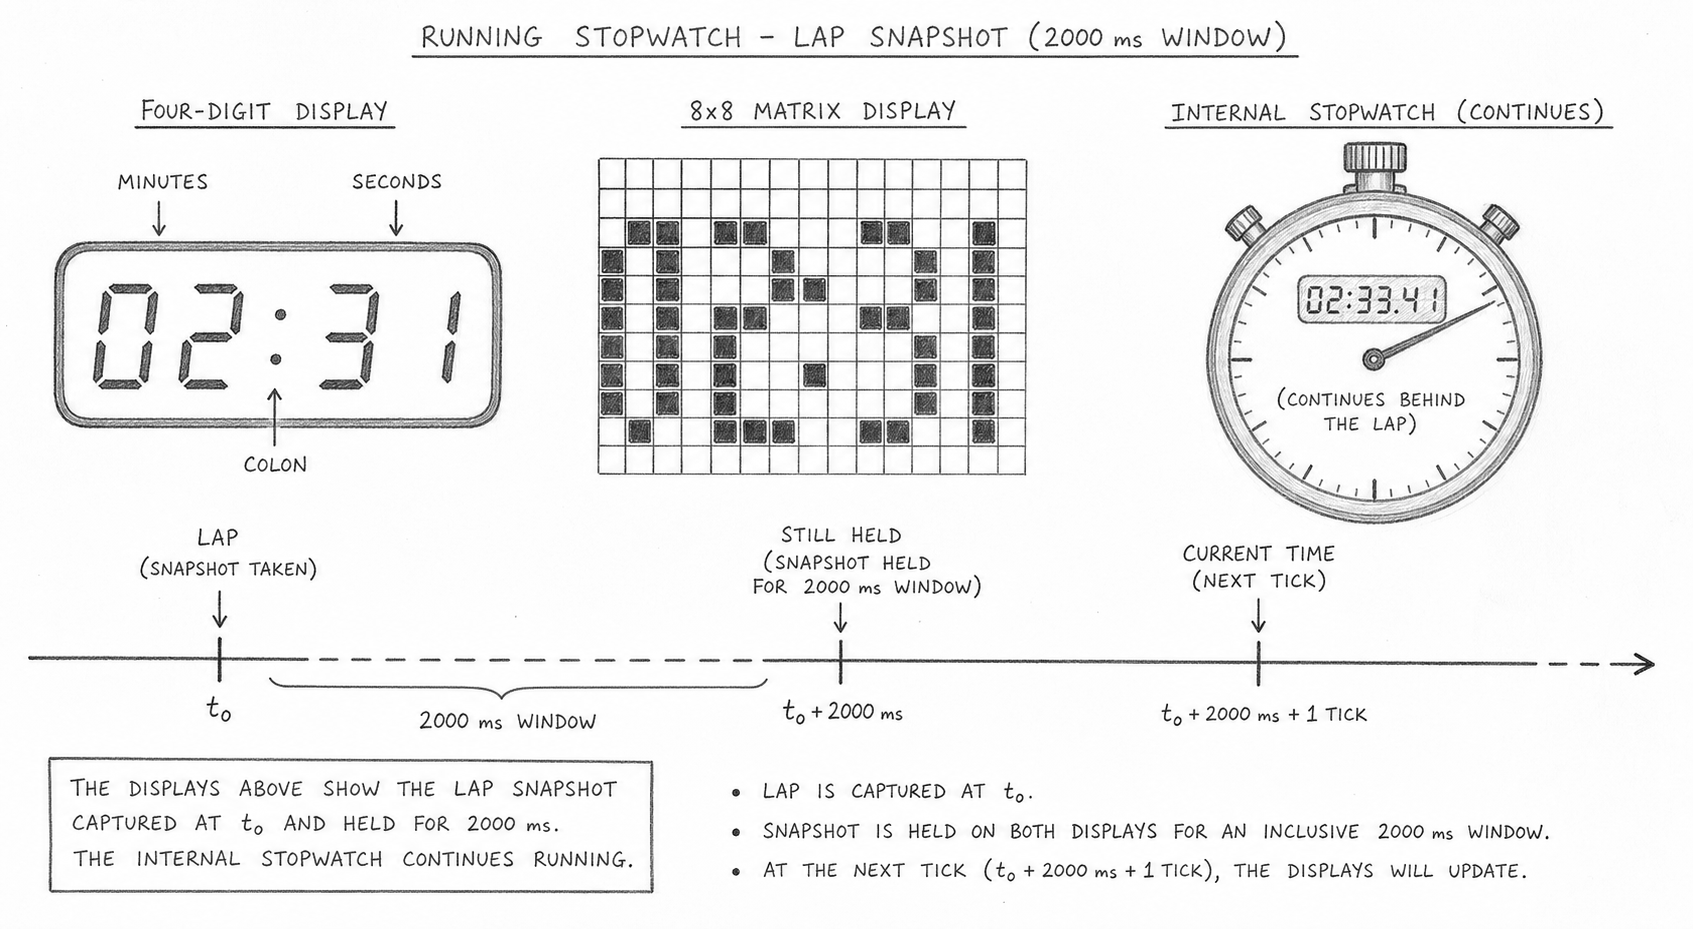
\includegraphics[width=0.95\linewidth,height=1.80in,keepaspectratio]
 {060-lap-hold-pencil.png}

\small\textit{Alternative text: a pencil timeline shows a lap snapshot pinned
above the two display cards through an inclusive two-second deadline while a
separate stopwatch line keeps moving; the next tick releases the pin and
freezes the newest current snapshot.}
\end{center}

\begin{tabularx}{\linewidth}{@{}l l l@{}}
\toprule
Elapsed & Four cells & Separator mask\\
\midrule
0 ms & 0:00.0 & \texttt{0x0A}\\
1 ms & 0:00.0 & \texttt{0x0A}\\
61,200 ms & 1:01.2 & \texttt{0x0A}\\
599,900 ms or greater & 9:59.9 & \texttt{0x0A}\\
\bottomrule
\end{tabularx}

\section{Draw the matrix dial from the same snapshot}
The matrix dial uses 28 perimeter pixels clockwise from the top-left corner:
across the top, down the right edge, back across the bottom, and up the left
edge without repeating corners. For
\(ms = elapsed \bmod 60000\), zero milliseconds lights no perimeter pixel.
Otherwise the count is
\(1 + \lfloor ms \times 28 / 60000 \rfloor\), capped at 28.

\begin{center}
% ADK visual: pencil
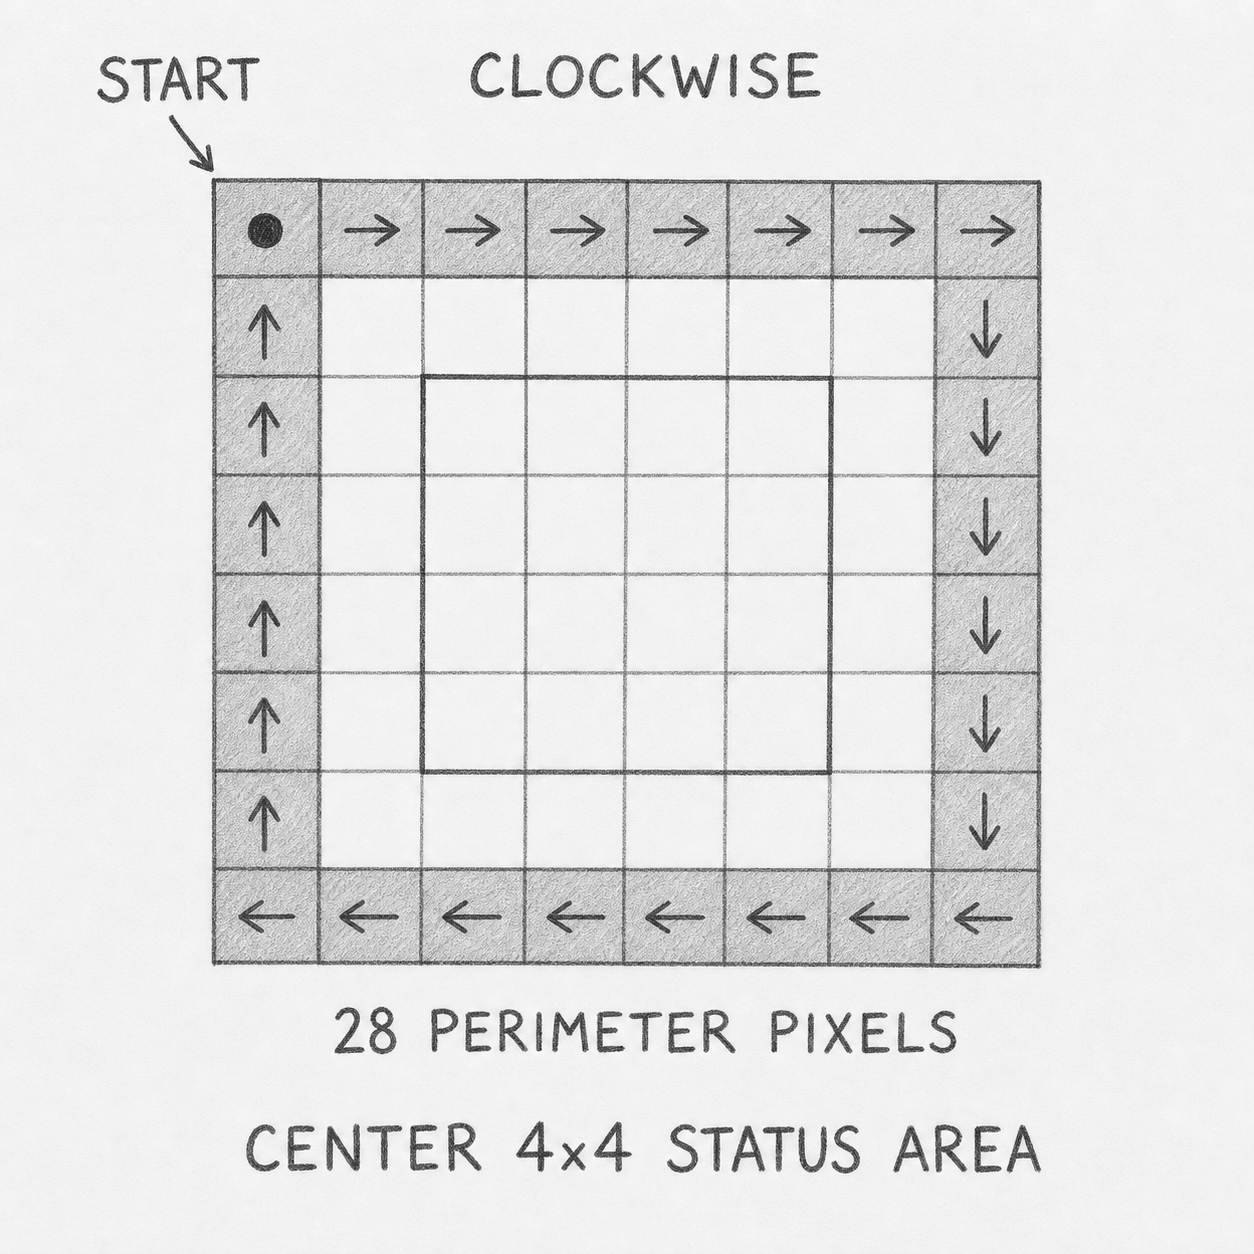
\includegraphics[width=0.94\linewidth,height=2.15in,keepaspectratio]
 {060-perimeter-dial-pencil.png}

\small\textit{Alternative text: a pencil eight-by-eight grid numbers the 28
unique perimeter pixels clockwise from the top-left corner, with arrows at
each corner and the central four-by-four area reserved for a status glyph.}
\end{center}

The first millisecond lights the first pixel. Every bucket boundary is fixed
by integer arithmetic. The final bucket lights all 28 pixels before minute
rollover; rollover returns the perimeter to zero.

\begin{tabularx}{\linewidth}{@{}l l X@{}}
\toprule
Time within minute & Lit perimeter count & Prediction to check\\
\midrule
0 ms & 0 & completely empty perimeter\\
1 ms & 1 & top-left pixel only\\
first bucket boundaries & golden integer counts & no floating-point drift\\
last millisecond & 28 & complete perimeter\\
60,000 ms & 0 & minute rollover\\
\bottomrule
\end{tabularx}

The central rows and columns two through five carry one four-by-four status
glyph. Its row nibbles are:
\begin{center}
\begin{tabular}{@{}l l@{}}
\toprule
State & Four left-to-right row nibbles\\
\midrule
stopped & \texttt{F, 9, 9, F}\\
running & \texttt{6, 3, F, 2}\\
paused & \texttt{A, A, A, A}\\
lap & \texttt{8, 8, 8, F}\\
fault & \texttt{9, 6, 6, 9}\\
\bottomrule
\end{tabular}
\end{center}
Lesson 059 orientation is applied only after the complete logical perimeter
and status frame exist.

\section{Publish one generation and wait}
Only one presentation generation may be outstanding. When none is pending,
the coordinator freezes the newest post-control stopwatch snapshot, derives
both frames, preflights both child policies, and commits both pure candidates.
The nonzero generation and its grace interval begin after both commits and
before the first child service.

While that generation is pending, supplied-time updates continue the internal
stopwatch. Presentation reports \texttt{ResourceBusy}; neither frame intent is
overwritten, and the caller must not replay an already admitted control edge.

\begin{center}
% ADK visual: pencil
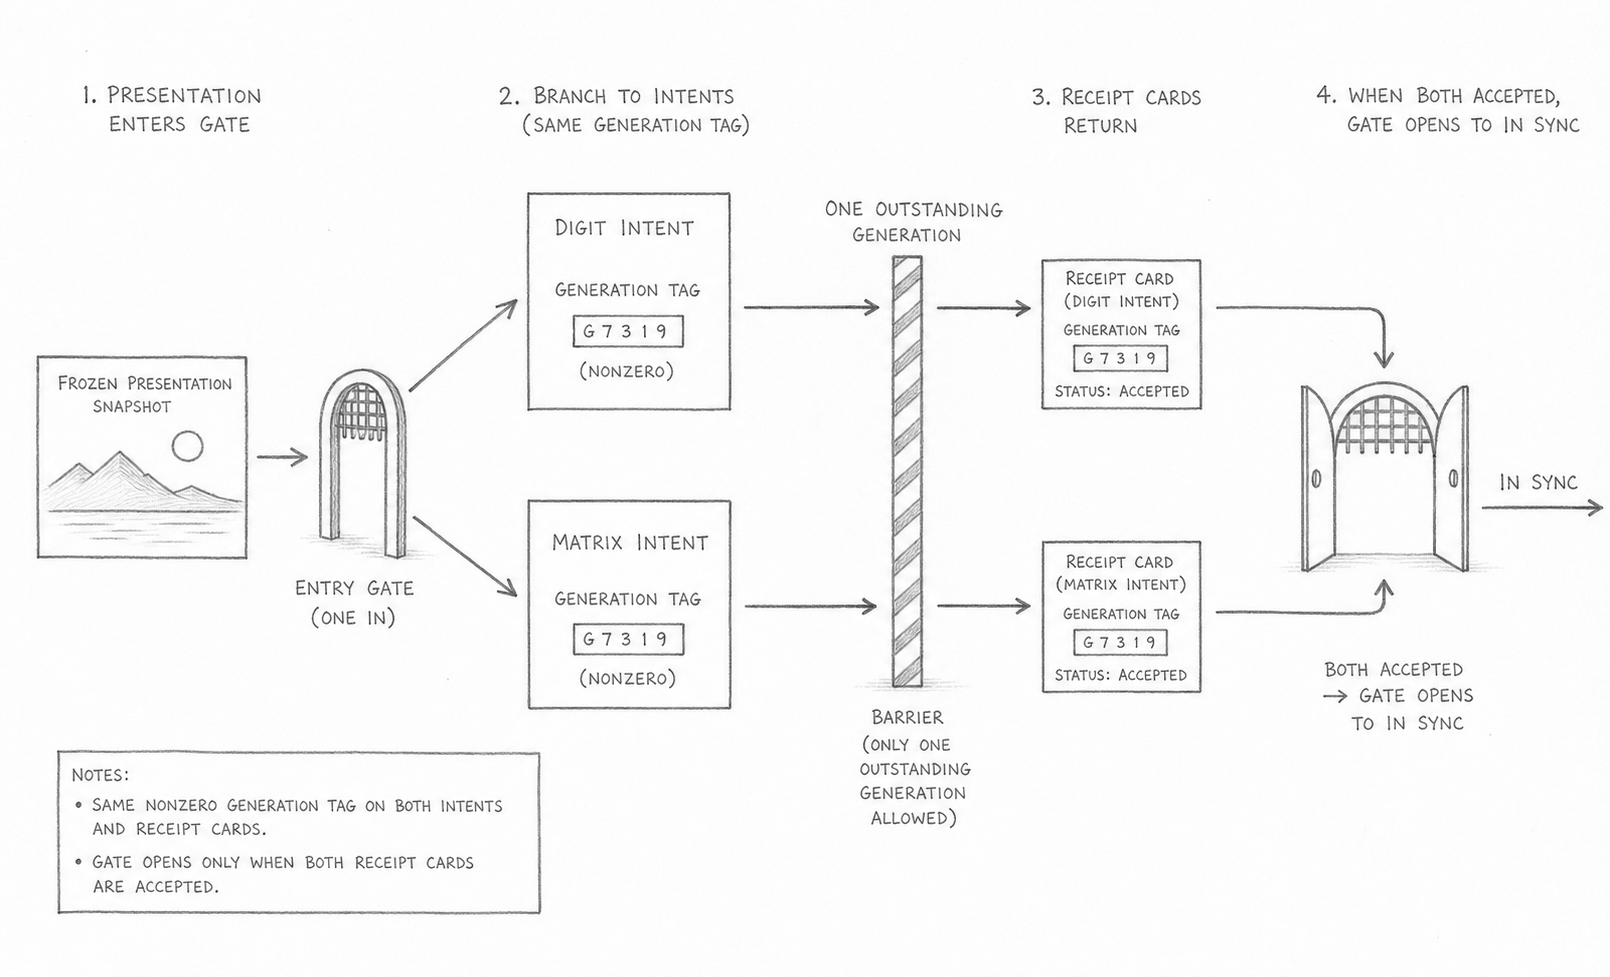
\includegraphics[width=0.96\linewidth,height=2.05in,keepaspectratio]
 {060-generation-gate-pencil.png}

\small\textit{Alternative text: one pencil generation card occupies a
single-slot gate and feeds separate digit and matrix acceptance checkboxes;
new stopwatch samples continue into a waiting latest-snapshot card but cannot
replace the occupied presentation card.}
\end{center}

\begin{lstlisting}
result = desk.update(envelope);
control = result.controlStatus;
presentation = result.presentationDisposition;
digits = result.digitTransaction;
matrix = result.maxCommand;
\end{lstlisting}

\texttt{controlStatus} and \texttt{presentationDisposition} are deliberately
separate. A presentation backlog must never make the caller repeat a control
edge that was already admitted.

\section{Correlate full receipts, not convenient hashes}
Each copied endpoint receipt carries owner, lifecycle, configuration,
requested and accepted generation, complete reported logical frame, reported
frame digest, status, blank-request acceptance, and observation time.
Generations are nonzero \texttt{uint32\_t} values with modular half-range
ordering and fault before wrapping to zero.

The digit and matrix sides use separate 32-bit FNV-1a digests. The domains are
\texttt{ADK.DIGIT.FRAME.V1} and \texttt{ADK.MATRIX.FRAME.V1}, encoded as ASCII
without a trailing NUL. The digit stream then alternates the one-byte numeric
glyph and one-byte diagnostic glyph for digit indices zero through three,
followed by the decimal mask, an overflow byte (\texttt{0x00} or
\texttt{0x01}), the source snapshot sequence, frame generation, and
presentation mode. The matrix stream instead follows its domain with rows zero
through seven, then the same source sequence, frame generation, and mode.
Both 32-bit integers enter least-significant byte first; the mode is one byte.
FNV-1a begins at \texttt{0x811c9dc5}, folds each byte separately, and
multiplies by \texttt{0x01000193} after each XOR.

\begin{lstlisting}
digit glyphs:      {0, 1, 2, 3}
diagnostic glyphs: {1, 2, 3, 4}
decimal / overflow: 0x0A / true
source / generation / mode:
  0x01020304 / 0x11223344 / 0x80
digit digest: 0x80dc784f

matrix rows: {0, 1, 2, 3, 4, 5, 6, 7}
matrix digest: 0x2887577e
\end{lstlisting}

The matrix witness uses the same source sequence, generation, and mode. These
literal results freeze both field order and little-endian integer encoding.

\begin{center}
% ADK visual: pencil
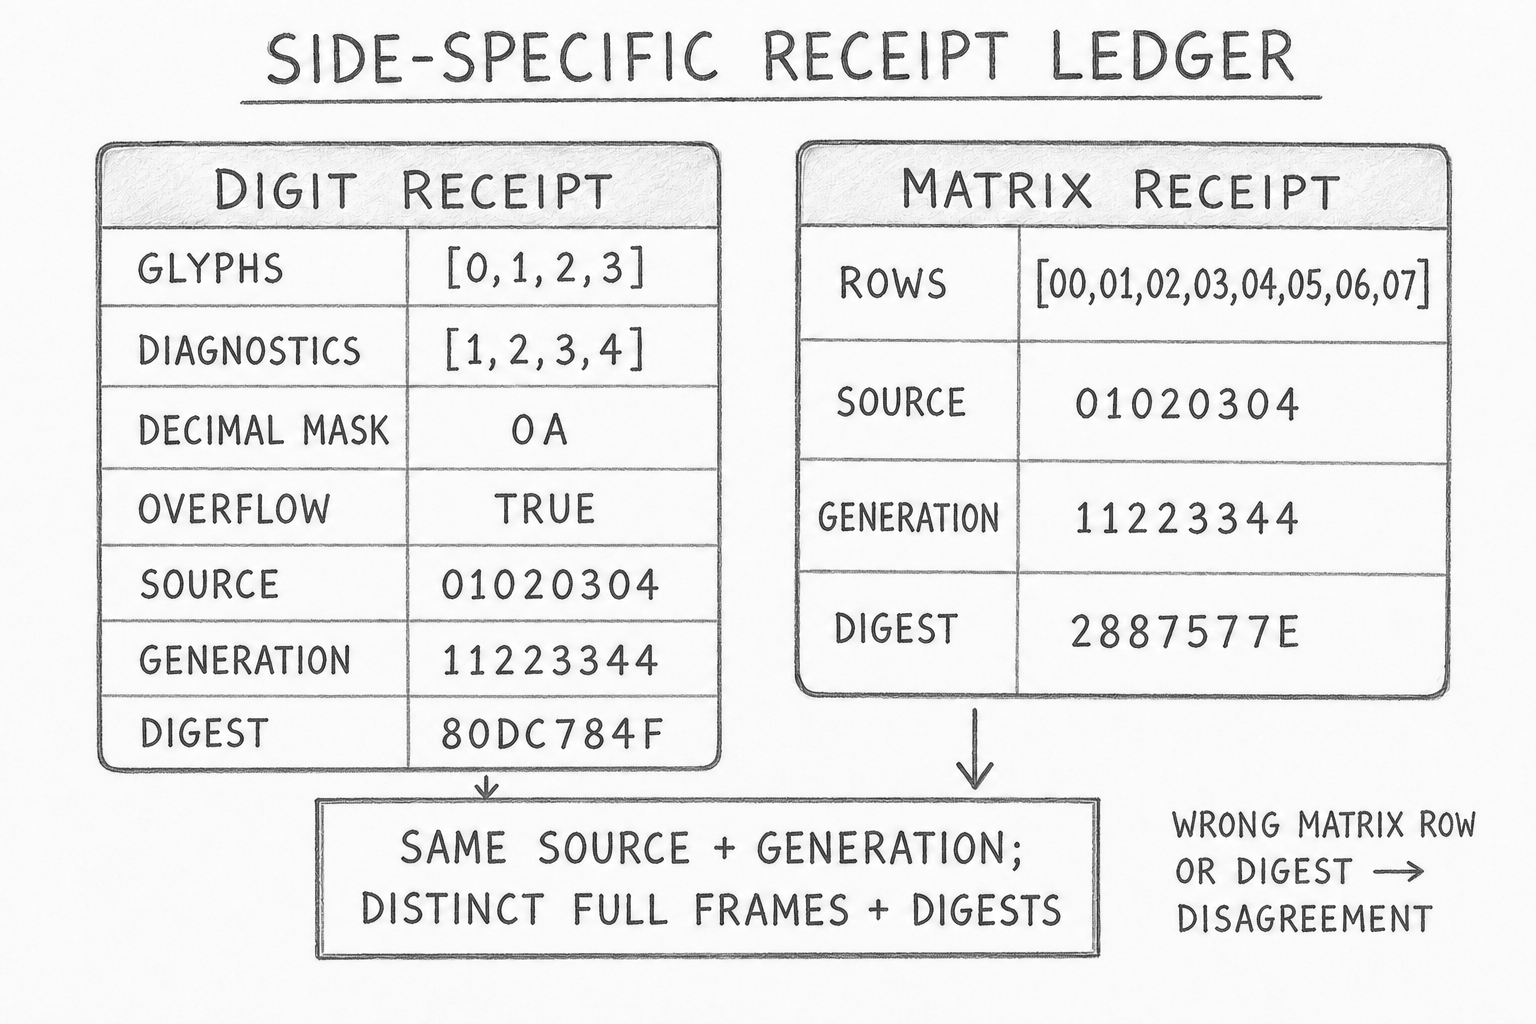
\includegraphics[width=0.95\linewidth,height=2.00in,keepaspectratio]
 {060-receipt-ledger-pencil.png}

\small\textit{Alternative text: separate pencil ledgers retain the complete
digit glyph, diagnostic, decimal-mask, and overflow frame and the complete
matrix row frame. Both carry source sequence 01020304 and generation
11223344, while their side-specific digests are 80DC784F and 2887577E. A
wrong matrix row or digest leads to disagreement.}
\end{center}

\lessonbox{\textbf{Digest rule.}
A digest is compact redundant evidence, not structural identity. Acceptance
requires the current generation, the side's expected digest, and byte-for-byte
agreement with the retained full frame.}

\section{Bound grace and name disagreement}
\texttt{presentationGrace} defaults to 100 ms and must be between 1 and
1,000 ms, well below modular half range. The generation remains pending
through the inclusive deadline and expires on the next valid tick.

\texttt{InSync} requires both sides to accept their own current generation,
digest, and complete frame. One accepted side and one pending side remains
pending during grace. Wrong digest, stale or crossed generation, one-sided
failure, digit refresh loss, or grace expiry enters presentation disagreement
with side-specific provenance. Stopwatch history is preserved, but both
displays receive blank requests.

\begin{center}
% ADK visual: pencil
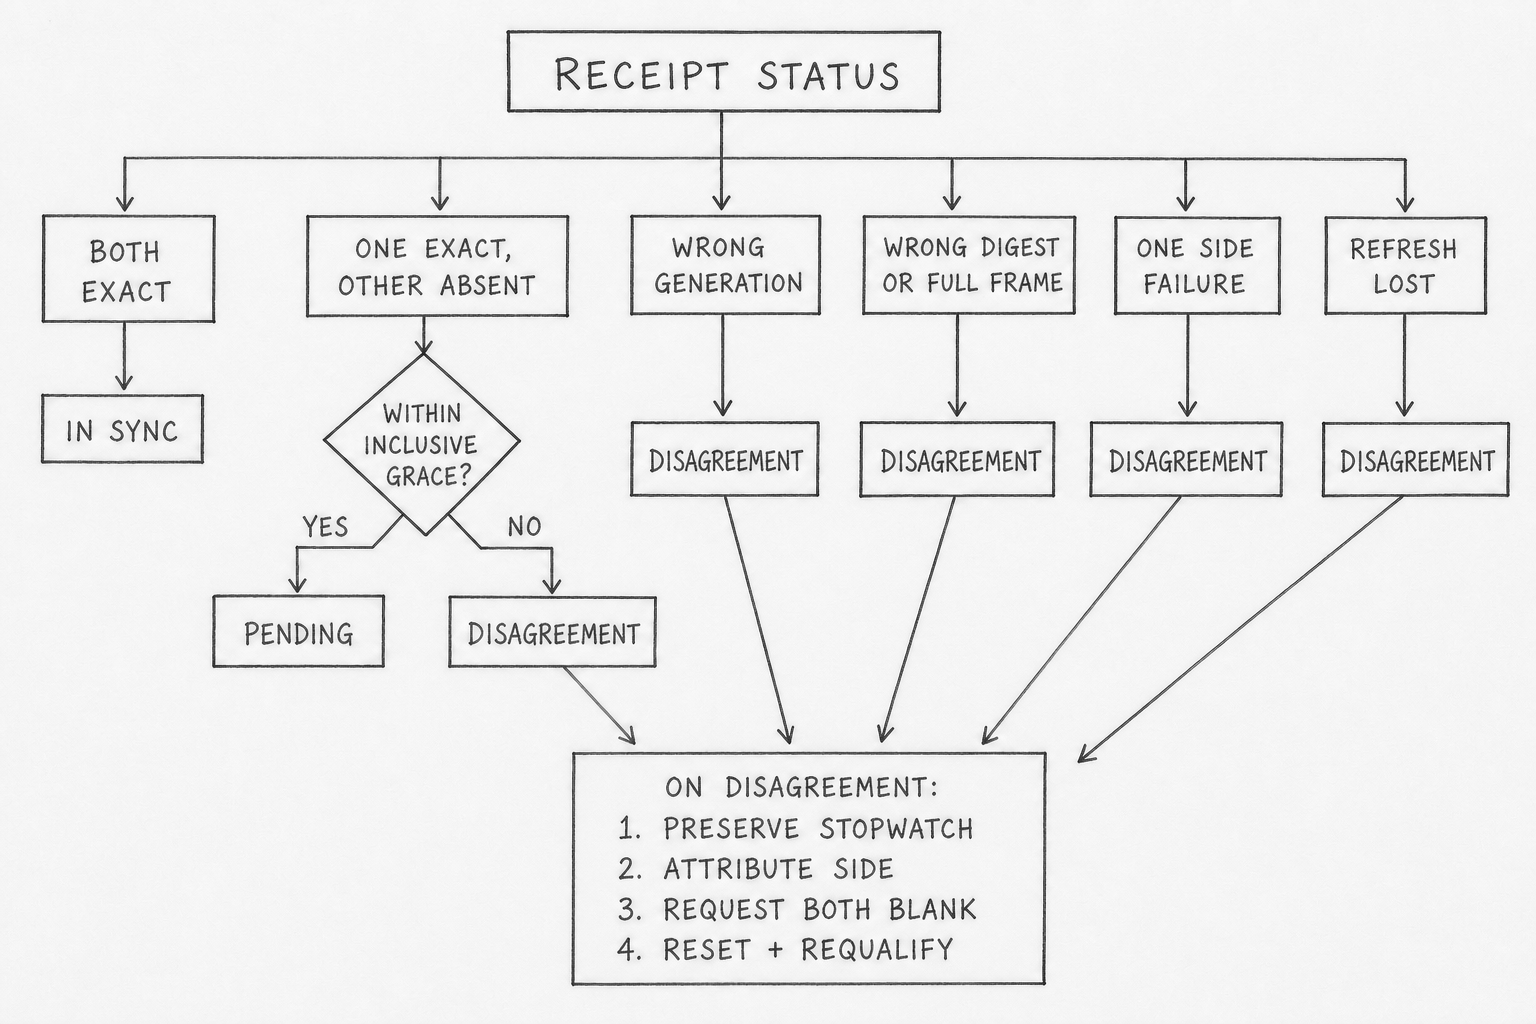
\includegraphics[width=0.96\linewidth,height=2.00in,keepaspectratio]
 {060-disagreement-pencil.png}

\small\textit{Alternative text: a pencil receipt-status decision tree keeps
one exact side and one absent side pending through the inclusive grace
deadline, reaches in-sync only through two exact matches, and routes late,
wrong-generation, wrong-frame, wrong-digest, failed, or refresh-lost evidence
to disagreement. Only disagreement requests both displays blank and begins
reset and requalification.}
\end{center}

\begin{tabularx}{\linewidth}{@{}X X X@{}}
\toprule
Evidence & Disposition & Next observation\\
\midrule
both exact current receipts & in sync & matching side generations and frames\\
one exact, one absent within grace & pending & inclusive deadline and missing side\\
wrong digest but matching full frame & disagreement & digest domain and byte order\\
right digest but changed full frame & disagreement & retained structural frame\\
digit refresh lost & disagreement & digit fault provenance and blank intent\\
next tick after grace & disagreement & anchored publication time\\
\bottomrule
\end{tabularx}

\section{Earn Ready through the common self-test}
Initialization does not jump directly to ordinary presentation. The
deterministic self-test has fourteen common stages: blank; eight indexed
segment-and-pixel stages; four digit-select-and-column stages; and final
blank. A stage advances only after both complete correlated receipts match its
generation and expected side-specific frame.

\begin{center}
% ADK visual: pencil
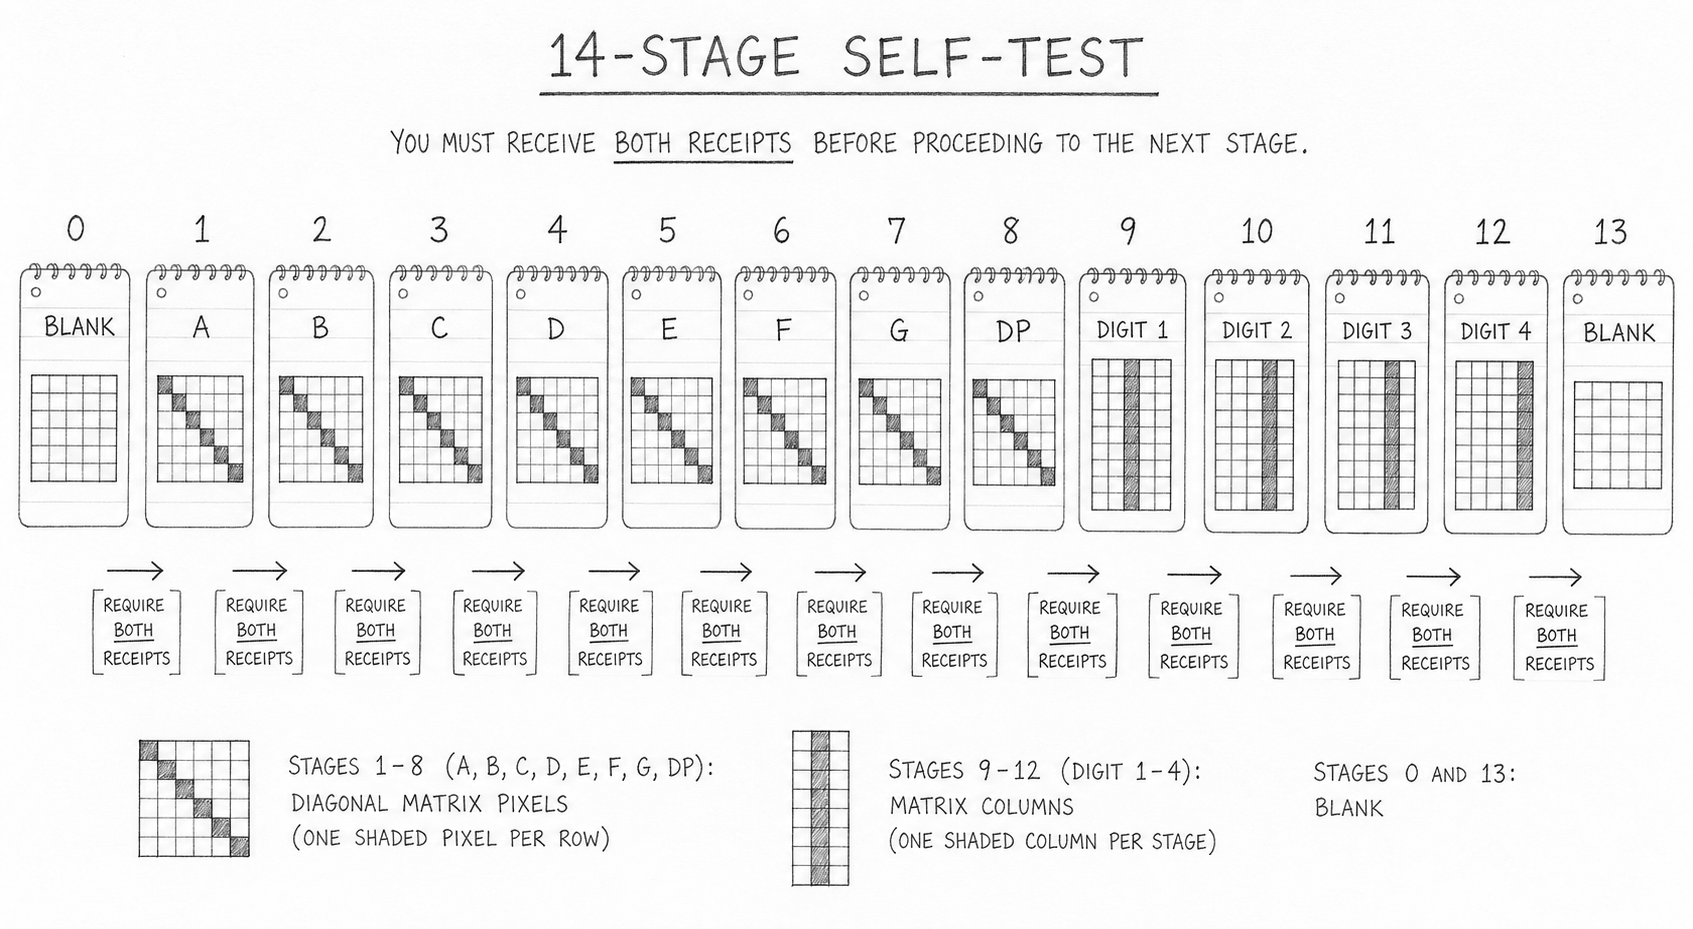
\includegraphics[width=0.96\linewidth,height=2.15in,keepaspectratio]
 {060-self-test-pencil.png}

\small\textit{Alternative text: a pencil strip of fourteen numbered cards
shows initial blank, eight cards pairing segment a through decimal point with
matching diagonal matrix pixels, four cards pairing one digit showing eight
with one matrix column, and final blank before a Ready gate.}
\end{center}

During the eight indexed stages, the digit policy lights segment \(a\) through
\(dp\) on digit \(index \bmod 4\), while the matrix policy lights pixel
\((index,index)\). During the four select stages, one digit shows 8 while the
matrix lights its matching column. \texttt{selfTestTimeout} is 100 ms per
stage: inclusive at the deadline, faulting on the next valid tick. Ready zero
is the first ordinary generation.

Predict which claim this E0 self-test supports: \longblank. Then name the
additional E1c observation required before saying the two physical displays
agree: \longblank.

\section{Follow one bounded service opportunity}
Every \texttt{update(envelope)} performs bounded work in a fixed order:
\begin{enumerate}
 \item validate the complete copied envelope;
 \item ingest child receipts;
 \item service one due digit transaction;
 \item service at most one MAX command;
 \item evaluate grace and self-test;
 \item apply valid control edges once;
 \item advance the internal stopwatch; and
 \item if no generation is outstanding, freeze, preflight, commit, and publish
       the next dual generation.
\end{enumerate}

Structural rejection mutates nothing. The caller must still service the
project often enough to satisfy Lesson 058's four-millisecond maximum digit
gap. No loop catches up missed scans or submits several MAX commands at once.

\section{Run the canonical replay}
Open
\texttt{examples/Lesson060DualDisplayTimingDesk/}\\
\texttt{Lesson060DualDisplayTimingDesk.ino}. Follow its narrative order:
\textbf{acquire} copied fixtures, \textbf{configure} timing and orientation,
\textbf{start} the self-test, then repeatedly \textbf{observe}, \textbf{decide},
and \textbf{present} at most one bounded service result.

Before running, record four predictions:
\begin{enumerate}
 \item The number of common self-test stages is \blankline.
 \item A valid lap edge is/is not replayed while presentation is busy:
       \blankline.
 \item Grace faults at the inclusive deadline/on the next tick:
       \blankline.
 \item The first ordinary Ready generation represents elapsed
       \blankline.
\end{enumerate}

After running, inspect named volatile result cells. Serial output may narrate
the trace, but it is never the sole evidence.

\begin{tabularx}{\linewidth}{@{}X X X@{}}
\toprule
Observation cell & Expected result & Interpretation\\
\midrule
self-test result & all fourteen stages correlated & Ready was earned logically\\
control result & admitted edge acts once & presentation busy is independent\\
digit result & one ordered refresh transaction at most & bounded scan service\\
matrix result & one register command at most & caller-paced transport\\
agreement result & two exact side receipts or named fault & no digest-only acceptance\\
shutdown result & both blank requests retained & logical safe intent only\\
\bottomrule
\end{tabularx}

\section{Diagnose the evidence boundary}
\begin{tabularx}{\linewidth}{@{}X X X@{}}
\toprule
Observed evidence & Likely policy meaning & Next check\\
\midrule
control OK, presentation busy & edge admitted while prior generation remains & do not replay control; service children\\
self-test stage does not advance & one receipt absent or mismatched & compare generation and full expected frames\\
digit side faults first & refresh deadline or receipt evidence failed & inspect digit provenance and service cadence\\
matrix side faults first & row sequence or copied receipt failed & inspect first MAX operation failure\\
both digests match, agreement fails & generation or structural frame differs & compare every receipt field\\
blank requested after fault & disagreement policy acted & do not claim physical darkness\\
\bottomrule
\end{tabularx}

\section{Keep the physical acceptance card open}
This lesson proves copied controls, supplied-time stopwatch behavior, coherent
dual frame generation, bounded child service, full-frame and digest
correlation, grace, self-test, disagreement provenance, restart, shutdown, and
compile-only Mega integration. It proves no electrical or optical behavior.

E1a must separately qualify the exact four-digit display, polarity, segment
and digit drivers, one resistor per segment, peak and aggregate current,
multiplex waveform, ghosting, and blank-on-release. E1b must separately
qualify the exact MAX7219 IC or module, schematic, RSET, decoupling, matrix
orientation, serial timing, current, startup, and shutdown. E1c may begin only
after both sides pass independently; it then measures combined supply demand,
timing interference, optical agreement, self-test visibility, fault blanking,
and simultaneous-current behavior.

\begin{center}
% ADK visual: pencil
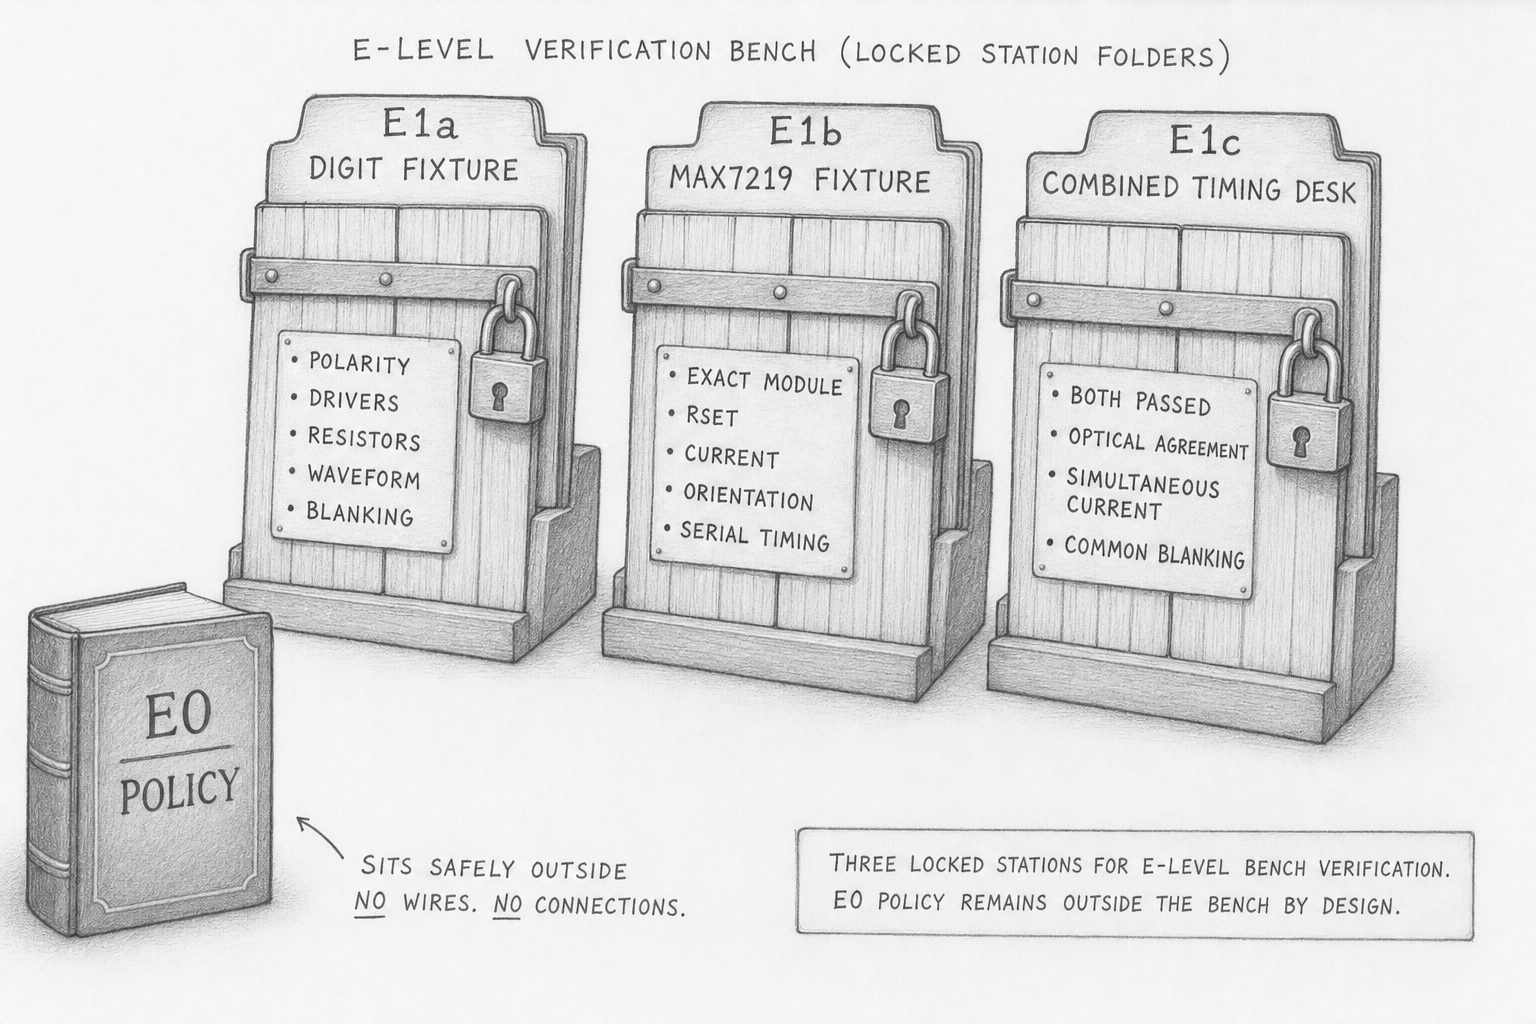
\includegraphics[width=0.95\linewidth,height=1.90in,keepaspectratio]
 {060-bench-gates-pencil.png}

\small\textit{Alternative text: three pencil laboratory cards remain stamped
OPEN: E1a qualifies the multiplexed digits, E1b qualifies the MAX7219 matrix,
and only arrows from both accepted cards permit E1c combined timing-desk
optical and current measurements.}
\end{center}

\begin{tabularx}{\linewidth}{@{}l X X@{}}
\toprule
Gate & Predict and observe & Acceptance record\\
\midrule
E1a resource & exact digit resources acquire and roll back & \blankline\\
E1a safe state & selects and segments release safely & \blankline\\
E1b resource & exact bus/device resources acquire and roll back & \blankline\\
E1b safe state & qualified shutdown and power-removal state & \blankline\\
E1c agreement & both displays visibly encode one snapshot & \blankline\\
E1c fault & one-sided failure drives observed safe response & \blankline\\
\bottomrule
\end{tabularx}

\section{Exit ticket}
\begin{enumerate}
 \item Why does one immutable presentation generation not promise
 simultaneous photons?
 \item Why are control admission and presentation disposition separate?
 \item What happens internally while a lap frame remains visible?
 \item Why must a receipt match both its digest and complete retained frame?
 \item When does the inclusive presentation grace interval expire?
 \item Which evidence must pass before the combined E1c timing desk may be
 powered?
\end{enumerate}

\lessonbox{\textbf{Completion evidence.}
You can replay every stopwatch phase, predict both frame mappings, trace the
fourteen-stage self-test, distinguish control admission from presentation
backlog, diagnose side-specific disagreement, and explain why copied logical
acceptance is not optical or electrical proof. Every physical acceptance card
remains explicitly open.}

\footnotesize
\textbf{Canonical companions:}
\href{https://github.com/spincyc/adk/blob/main/examples/Lesson060DualDisplayTimingDesk/Lesson060DualDisplayTimingDesk.ino}{Lesson 060 sketch}
\quad
\href{https://github.com/spincyc/adk/blob/main/site/pages/lessons/060.md}{HTML lesson source}
\quad
\href{https://github.com/spincyc/adk/blob/main/docs/design/LESSONS_058_060_DISPLAY_TIMING_DESK_PLAN.md}{implementation plan}
\end{document}
